% DUET -- Background and Motivation (DAC 2027 draft, 2026-10-21)
% Numbers: raw I/O = 128K-aligned uniform random replay at QD32 (results/final_rp_a128), 1/8 mapping DRAM, OP 7%.
% Figure: results/paper_dac/fig_motiv.pdf (tools/plot_motiv.py).

\section{Background and Motivation}
\label{sec:bg}

\subsection{Address Translation under a DRAM Budget}
A page-level FTL keeps one entry per 4\,KiB logical page, so its table is
about 0.1\% of the capacity and grows linearly with it. When the controller
DRAM can hold only a fraction of this table (1/8 in this paper), the FTL must
either keep part of the mapping in flash or map data in larger units. The
three approaches below take these two routes, and each one moves the cost to a
different part of the I/O path.

\textbf{On-demand mapping.}
DFTL~\cite{dftl} stores the whole page-level table in flash as translation pages
and caches recently used entries in DRAM; a small global directory locates each
translation page. A read whose entry is not cached must first read the
translation page and only then the data page, so two flash reads are
serialized on the read path. Evicting a dirty entry also writes its translation
page back, which adds write amplification. LeaFTL~\cite{leaftl} compresses the
cached mapping into learned linear segments, so the same DRAM covers more pages.
The segments, however, are built only from runs of sequentially placed pages,
and a mispredicted location costs an extra flash read. For data written randomly
or reordered by garbage collection, both FTLs miss often, and every miss turns
one read into two dependent flash reads. Read latency therefore depends on the
cache hit ratio, not on the device.

\textbf{Traditional hybrid mapping.}
Hybrid FTLs such as BAST~\cite{bast} and FAST~\cite{fast} map most data per erase block,
which needs only one entry per block, and absorb updates in a small pool of
page-mapped \emph{log blocks}. When the pool runs out, a log block is reclaimed
by \emph{merging}: for each logical block that has pages in it, the valid pages
from the data block and the log blocks are copied into a fresh block, and the
old blocks are erased. In FAST a log block is fully associative, so one
reclamation can trigger a full merge for every logical block that it touches.
Reads stay cheap, because the block map always fits in DRAM. Merges, however,
run on the write path when no log block is free, so the write that triggers
them waits for several block copies. Each merge copies up to a whole erase
block, and erase blocks keep growing with every 3D NAND
generation~\cite{TODO-block-size}. The result is long write stalls (write
latency) and many extra copies (write amplification), which together lower
write bandwidth.

\textbf{Large-IU mapping.}
High-capacity SSDs in production avoid both problems by using a large
\emph{indirection unit} (IU) of 16--64\,KiB~\cite{TODO-iu}. One entry per IU
shrinks the table by the IU size over 4\,KiB, so the whole table fits in DRAM:
every read takes a single flash access, and there are no block merges. The cost
moves to writes smaller than an IU. The FTL must read the rest of the unit,
merge the new data, and program the whole unit again (read-modify-write, RMW).
The extra reads lengthen the write path, and the rewritten pages raise write
amplification by up to the IU size over the write size. In our evaluation the
1/8 budget allows a 32\,KiB IU (4\,B per 32\,KiB).

\subsection{Motivation}
Figure~\ref{fig:motiv} compares the three approaches with a page-level FTL
that keeps its whole table in DRAM. All FTLs run in NVMeVirt~\cite{nvmevirt}
with the same NAND timing and the same 1/8 mapping-DRAM budget. The workload is
uniform random I/O over the whole device at 50\% reads; 70\% of the requests are
4\,KiB and the rest 128\,KiB, each aligned to its own size (QD32).

\textbf{On-demand mapping slows reads.}
With mapping misses, DFTL needs 1.73 flash reads per host read and LeaFTL 1.32
(Figure~\ref{fig:motiv}a; LeaFTL's misprediction reads are not counted, so its
value is a lower bound). Their average read latency is 2.3$\times$ and
1.4$\times$ that of the page-level FTL (Figure~\ref{fig:motiv}b), although the
flash itself is the same.

\textbf{Hybrid mapping and large IUs slow writes.}
FAST's block merges raise WAF from 8.6 to 26.5 (Figure~\ref{fig:motiv}c) and
stall writes, so its average write latency is 3.0$\times$ that of the page-level
FTL (Figure~\ref{fig:motiv}d) and it delivers only 34\% of the page-level
throughput. The large IU avoids merges, but every 4\,KiB write becomes an RMW of
its 32\,KiB unit: WAF reaches 12.8 (1.5$\times$) and write latency grows by 1.4$\times$.

DUET, shown for reference, uses the same 11.2\,MB as the other bounded FTLs
(1/8 of the page-level table), serves every read here with one flash read, and stays within
1.1$\times$ of the page-level FTL in average read and write latency and WAF.

\textbf{Goal.}
An FTL that fits a limited DRAM budget should therefore (i) minimize mapping
reads, so that a host read costs a single flash read as with a large IU,
(ii) eliminate block merges, and (iii) absorb small writes without RMW.
DUET meets all three by keeping the large IU and adding a fine-grained level
whose mapping is elastic.

\begin{figure}[t]
  \centering
  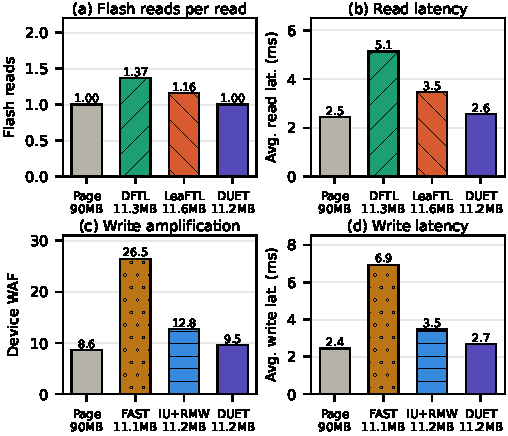
\includegraphics[width=\columnwidth]{figs/fig_motiv.pdf}
  \vspace{-6mm}
  \caption{Cost of existing FTLs under a 1/8 mapping-DRAM budget (uniform random,
  50\% reads, 70\% 4\,KiB / 30\% 128\,KiB size-aligned requests, QD32). (a)--(b)
  On-demand mapping; (c)--(d) block-level hybrid (FAST) and a 32\,KiB IU with RMW.
  Latencies are averages. Labels give each FTL's mapping DRAM. Page: page-level
  FTL with the full table in DRAM; DUET (Section~\ref{sec:design}) shown for reference.}
  \label{fig:motiv}
  \vspace{-3mm}
\end{figure}
